\subsection{Code analysis}

The code was analysed via the use of JadX, the program was able to decompile the code and present it in a readable manner. 
Many parts of the code however like classes were obfuscated via the use of hashes. 
Some of the functions and classes were readable and gave some clue of what they could represent. 
Via this method a local database function was found which saves the users settings as shown on figure \ref{tim-database}.

\begin{figure}[H]
    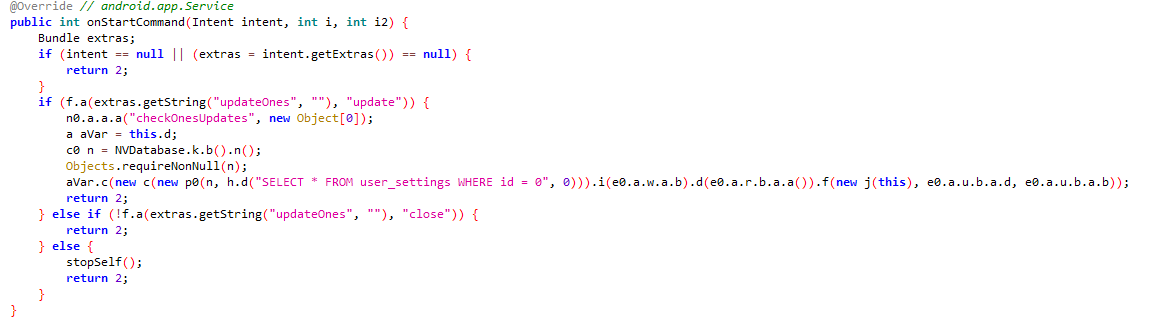
\includegraphics[width=1\textwidth]{codedatabase.PNG}
    \caption{Database hidden in the code}
    \label{tim-database}
\end{figure}